\documentclass[a4paper,12pt, oneside]{book}
\usepackage{ecsp}
\usepackage{hyperref}
\hypersetup{
	colorlinks,
	citecolor=black,
	filecolor=black,
	linkcolor=black,
	urlcolor=black
}

\makeindex



\begin{document}

%\author{Kenneth Carter Dodd}
%\title{Essentials of Computer Science Principles\\ with JavaScript}
%\date{2015}



%\frontmatter
%\maketitle

\begin{titlepage}

\begin{center}
	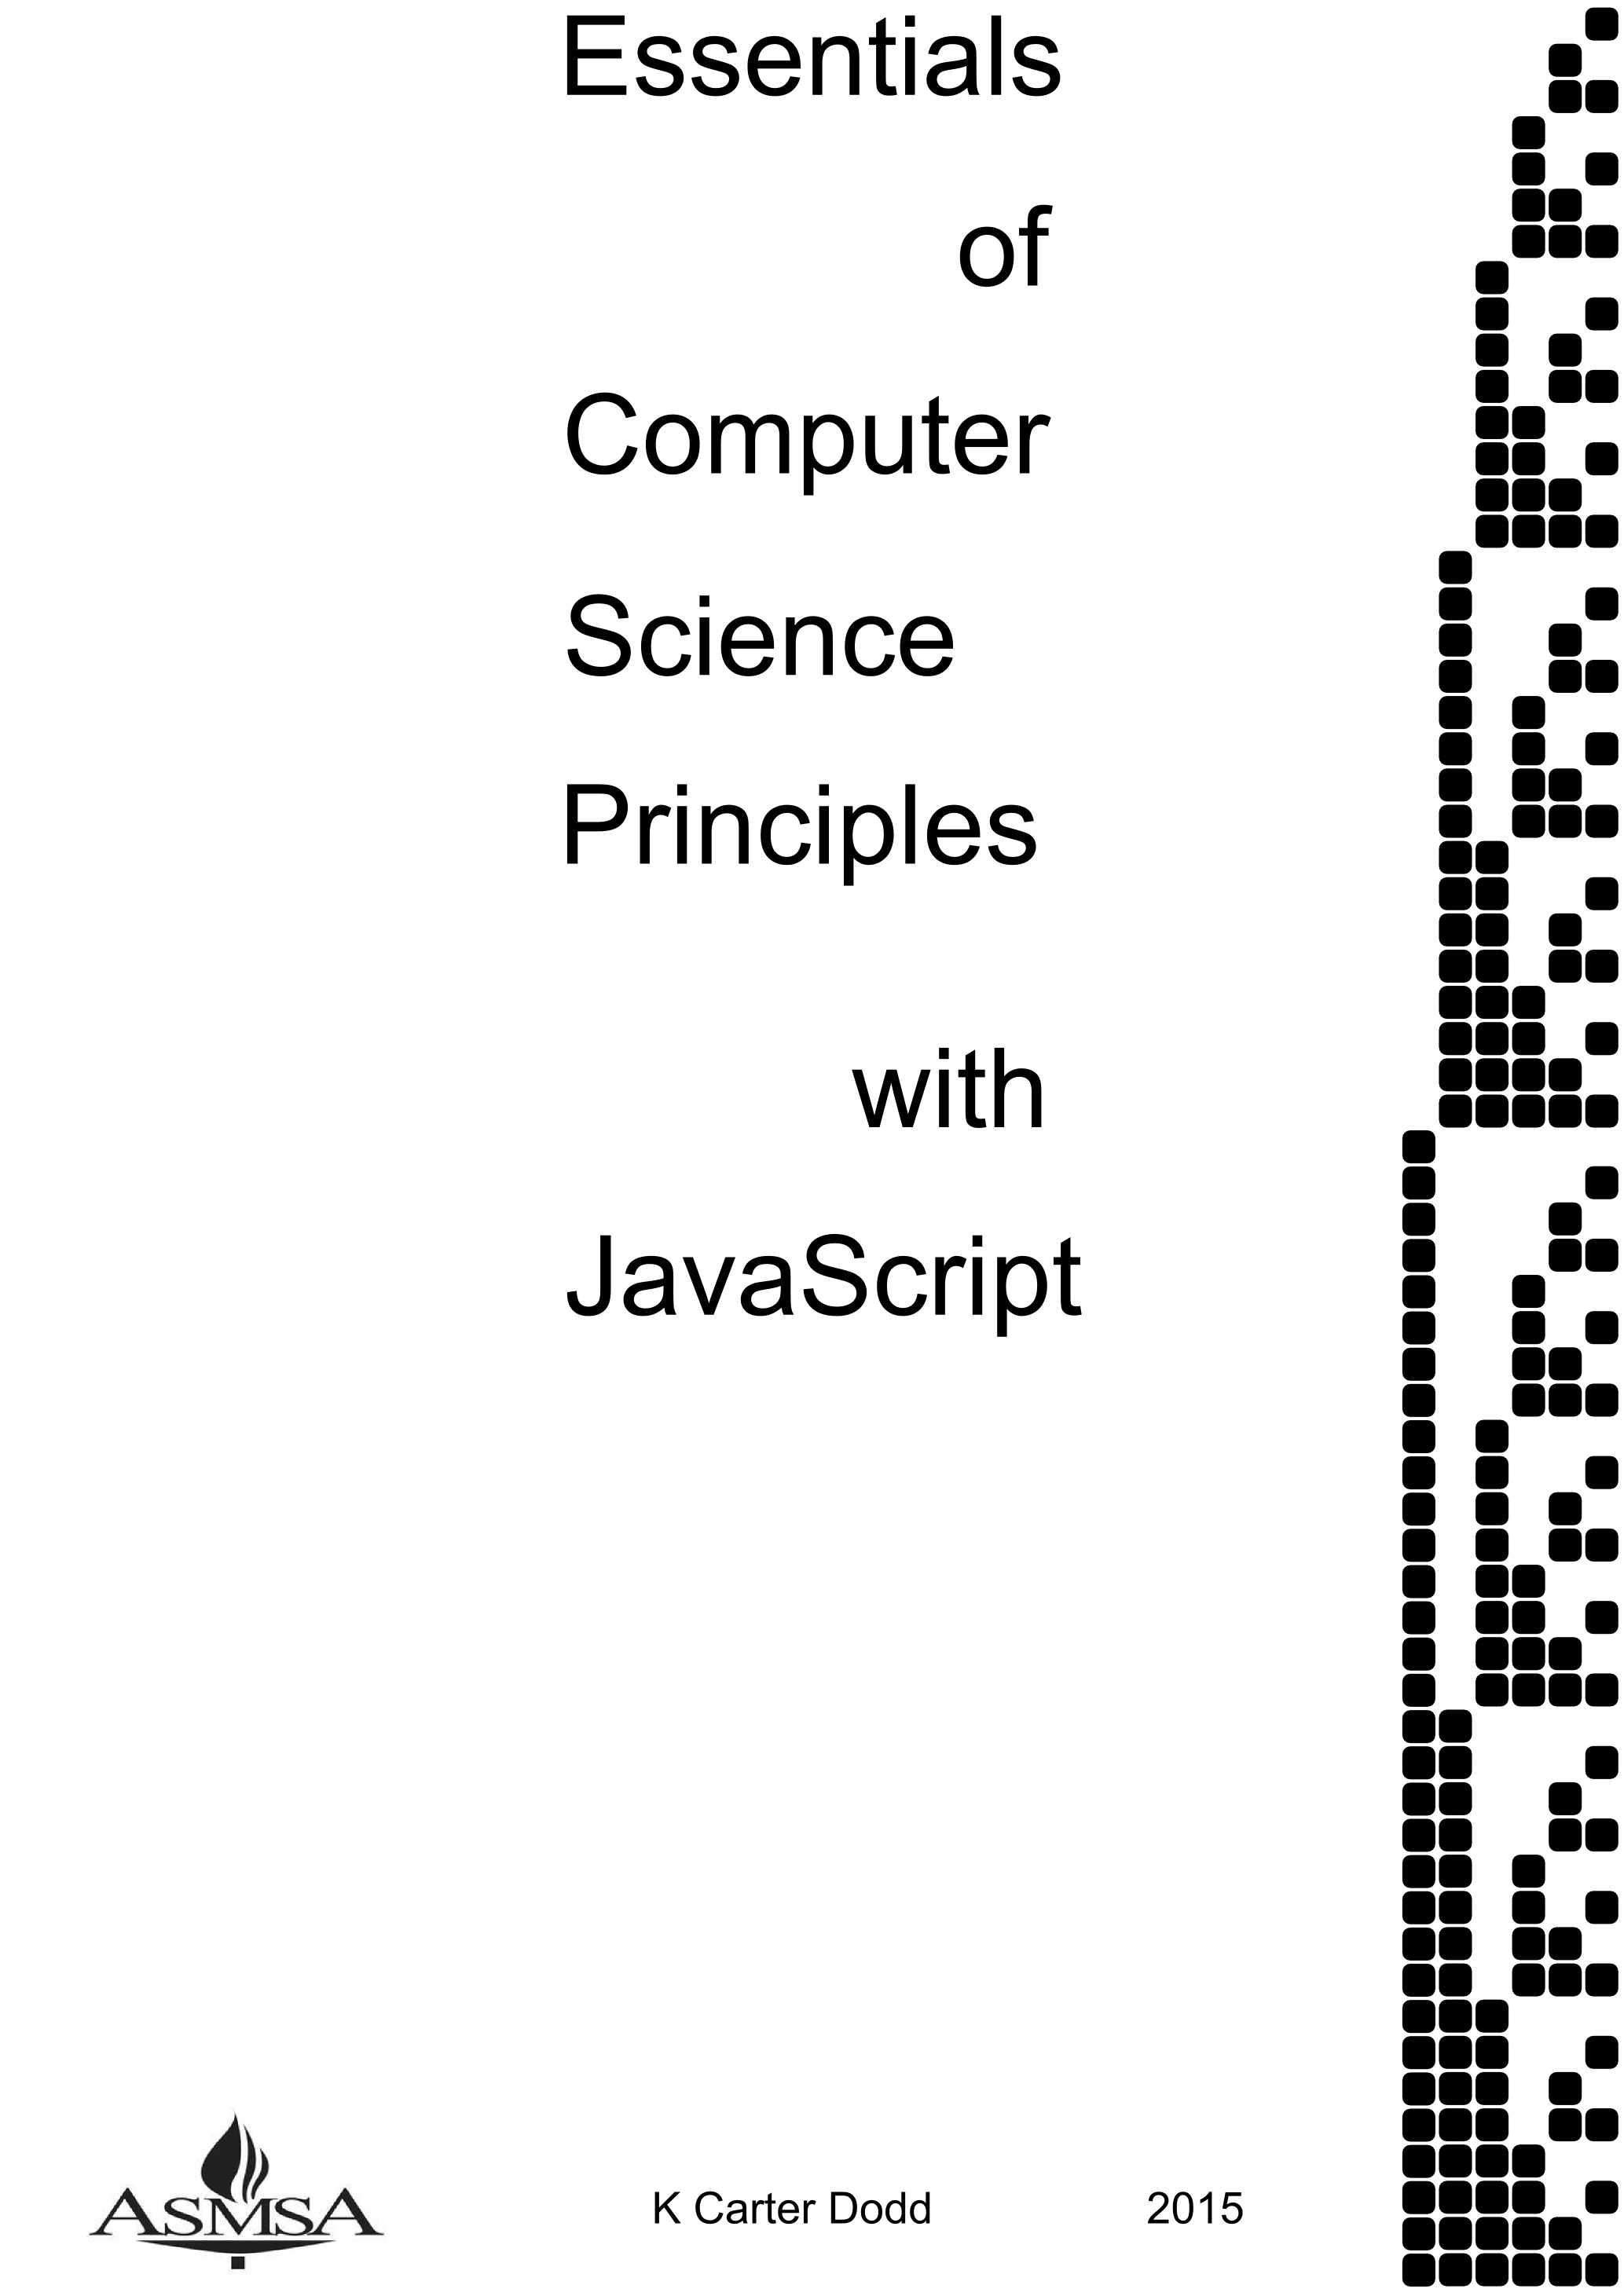
\includegraphics[width=\textwidth]{./images/cover.png}
\end{center}
\end{titlepage}

\frontmatter
\tableofcontents

\mainmatter
\chapter{Computation}

What do we mean by computation? In a very general sense, a computation is a goal that is possible to reach by some number of intermediate steps. You may be familiar with doing computations in math, such as multiplying two numbers. But the idea of computing is much broader than your math class. Any problem that \textit{can} be broken down into specific steps to reach a specific conclusion is called computable. The details of the exactly what steps to take in a computation is called an \textbf{algorithm}. Figuring out how to combine things that you \textit{can} do to accomplish something you can't do yet is the essence of computer science.\\

\section{Sequence of Instructions}

For example, think about how you follow directions when traveling from one location to another. The first time you go somewhere you probably need to either ask someone how to get there, or follow the directions of a GPS device or a map. The ultimate problem is to go from A to B. Directions might come in the form of turning left or right on a particular street, then following that street for some distance, then making another turn, and so on.\\

\index{sequence}

Solving the problem of going from A to B can be broken down into some number of simpler problems. You don't need anyone to explain how to turn left/right or follow a street because you already know how to accomplish those tasks. All you need to know is what order, or sequence, to do them in to get to where you're going.\\

A electrical/mechanical computer starts with a very limited number of instructions that it can understand, and 'knows' how to accomplish. What we have to do is to figure out how to accomplish more complicated actions by breaking them down into a larger number of simpler ones until we are \textit{only} telling the computer those that it can understand.

\begin{center} \imagegraphic[1.0]{mapA.png}\end{center}

Come up with a sequence of instructions to give someone that doesn't have the map. They will start at A, and want to arrive at B. As an example, consider these instructions starting at A. Which location would you arrive at?

\begin{description}
	\item[] Go north.
	\item[] Turn right when you reach Market St.
	\item[] Go several hundred feet then turn right again.
	\item[] Go down the street and it's on the left.
\end{description}

Is the set of instructions specific enough to get there? Would the instructions be different if the person didn't know which way was North, or was a poor judge of distance? How can the instructions be altered to be more robust?\\

\section{Instruction Set}

\index{instruction set}

One issue with the problem of giving someone a sequence of instructions is that we need to know a little more about what they know how to do, so that we know what kind of instruction we need to give them, and how specific we need to be.\\

Before we start listing the sequence of instructions, we should write down what instructions we have to work with: the instruction set. Suppose we came up with the following set of instructions to choose from, and using the \# symbol to mean we can use that instruction with any number substituted in for \#.\\

\textbf{Directions Instruction Set}
\begin{itemize}
	\item Turn Left.
	\item Turn Right.
	\item Go Forward \# feet.
\end{itemize}
	
What would the directions look like now if we could only use some sequence of these instructions? Lets assume the person will start out facing the road, wherever they begin, and let's tell them how to go from A to B using only these instructions. One sequence might be the following.

\begin{description}
	\item[] Turn Right.
	\item[] Go Forward 200 feet.
	\item[] Turn Left.
	\item[] Go Forward 200 feet.
	\item[] Turn Right.
	\item[] Go Forward 100 feet.
\end{description}

\index{variable}

We could make this more compact by coming up with codes to represent each instruction, along with a definition of what that code means. Instead of using the \# sign to represent any number, I am going to list what is supposed to represent this number with what is called a variable inside parenthesis of the codes. If there is no variable for that instruction, then there is nothing listed inside the parentheses. When the code for instruction is used we can replace the variable with the number we want to use for it.\\

\textbf{Directions Instruction Set Codes}
\begin{description}
	\item[L()] : Turn Left.
	\item[R()] : Turn Right.
	\item[U()] : Make U-turn.
	\item[F(x)] : Go Forward x feet.
\end{description}

Now the sequence of instructions would look like the following.

\begin{description}
	\item[] R()
	\item[] F(200)
	\item[] L()
	\item[] F(200)
	\item[] R()
	\item[] F(100)
\end{description}

\section{Abstraction}

\index{abstraction}

Think about this. Once they know how to go from A to B, then you don't need to tell you how to get there anymore. Suppose now they need to go to location C. You could tell them to go from A to B first, then give further instructions of how to go from B to C. We can alter the instruction set by defining a new instruction to go from A to B using the codes for the other instructions that they already know.\\

\begin{description}
	\item[AB()] : go from A to B using the following
	\begin{description}
		\item[] R()
		\item[] F(200)
		\item[] L()
		\item[] F(200)
		\item[] R()
		\item[] F(100)
	\end{description}
\end{description}

Now I can write a sequence of instructions to go from A to C using this new instruction AB(). The details of how to get from A to B are now \textit{abstracted}, which makes writing more complicated directions easier.
\begin{description}
	\item[AC()] : go from A to C
	\begin{description}
		\item[] AB()
		\item[] F(100)
		\item[] L()
		\item[] F(500)
	\end{description}
\end{description}

\section{Conditional Instructions}

So far we have created instructions that are intended to be followed, in order, no matter what. But in practice we know that not everything can be described quite that simply. What use would the instructions be if the road was blocked off for construction? We may not know that ahead of time, so we need to be able to prepare our instructions to handle that possibility.\\

The idea of a condition is that one set of instructions will be followed if the condition is true, but a different set of instructions should be followed if it is false. Here the condition might be, "Can you move forward?". If they can, then they can move forward down the road, but if they can't we need to give alternative instructions of what to do from that point on.\\

We can come up with a codes for following conditional instructions, just like for other instructions. However, instead of the codes telling us where to go in the map, it tells us where to start reading other instruction codes. The IF-ELSE code says that if a condition is true, the instructions immediately following the IF code are followed. But if the condition is false, the instructions immediately following the ELSE code are followed instead.\\

Suppose we give the same instructions as above, but we know that sometimes Broadway St. is sometimes closed to traffic. We can build in a condition that if when the driver gets to Broadway and it's closed, they can go an alternate rout. The condition is "Is Broadway St. open to traffic?". If the answer to that is 'yes', we follow the normal instructions. But if it is 'no', then we follow the instructions under the ELSE code until the ENDIF code is reached. \\

\begin{description}
	\item[AC()] : go from A to C
	\begin{description}
		\item[] AB()
		\item[] F(100)
		\item[IF]: Is Broadway St. open to traffic?
		\begin{description}
			\item[] L()
			\item[] F(500)
		\end{description}
		\item[ELSE]:
		\begin{description}
			\item[] U()
			\item[] F(200)
			\item[] R()
			\item[] F(300)
			\item[] R()
			\item[] F(500)
			\item[] L()
			\item[] F(200)
		\end{description}
		\item[ENDIF]:
	\end{description}
\end{description}

\section{Flowchart}

A flowchart is a way of organizing this conditional nature of the directions in a visual way. Here, boxes are the individual directions, and the diamond is the condition which has two possible set of directions. Visualizing the instructions this ways shows that an algorithm itself is like a map, with more than one possible path depending on what is true during any given time through the algorithm. Describing the algorithm using codes or the flowchart are made completely analogous to each other. Flowcharts can be used to plan out an algorithm before implemented with a specific set of codes.\\

\begin{center} \imagegraphic[0.5]{flowchart.png}\end{center}

\section{Iteration}

If a conditional statement results in repeating a previous set of instructions, it is called an iteration. This can be visualized using a flowchart. Suppose instead of having to measure the distance needed to drive after each turn, we want to tell the driver to simply drive until an intersection is reached.\\

We can have a conditional block asking whether or not they are at an intersection. If not, then drive forward some more. If they are, then make the required turn. This will result in what is called a loop. "Are you at an intersection?" serves as the loop condition, which causes the loop to keep repeating until the driver arrives at an intersection. \\

\begin{center} \imagegraphic[0.5]{iteration.png}\end{center}

Perhaps we would like to check to see if they are at an intersection before driving forward, instead of afterward. The main difference is that if the driver is already at an intersection, they can go ahead do the next instruction without having to drive forward (which might cause them to miss the turn).\\

\begin{center} \imagegraphic[0.5]{iteration2.png}\end{center}

\section{Sequence, Condition, Iteration}

Any algorithm can be described using some combination of these three basic control structures. When creating a programming language, we must ensure that these functions are possible to describe and implement within the language so that any algorithm can be written using that language. To make the set of codes for driving directions complete, we really need a way to do iteration. The WHILE code will be used to do this.\\

As long as the condition associated with the WHILE statement is true, the instructions immediately following the while statement are followed, and then the condition is reconsidered. When the condition is false, the instructions under the WHILE statement are no longer followed, and instead the instruction after the ENDWHILE code is followed.\\

The while loop could be used to define a generic 'forward' code. Since we want it to repeat when the driver is not at the intersection, we have to change the question slightly.\\

\begin{description}
	\item[F()] : go forward until intersection is reached.
	\begin{description}
		\item[WHILE]: Are you not at an intersection?
		\begin{description}
			\item[] F(100)
		\end{description}
		\item[ENDWHILE]:
	\end{description}
\end{description}

This is how programming languages start to be developed. Once some basic operations, or instructions, are built in to the language, many other and more complicated operations can be built using them.
\chapter{Logic and Binary Arithmetic}


\chapter{Arithmetic}

You are probably somewhat familiar with doing various forms of arithmetic, and have probably even memorized the results of many operations. But the idea in computer science is to break down that process into a sequence of steps called an algorithm. It is important to understand that there are multiple possible algorithms to accomplish the same result. Remember that an algorithm is a set of directions to a destination, but the same destination can have several possible routes.

\section{Addition and Subtraction}

Let's start simple with the addition of two digits. Like 1+1, or 2+5. You probably don't even need to think about how to do these, you just know the answer. But I want you to think about how to explain what is going on as an algorithm. Something you might not even think about anymore is why do these symbols 1, 2, 3, ... mean anything? We simply memorize their meaning, and the symbol itself does not have any intrinsic value.\\

Let's start by adding 1 to any of the 10 digits (0, 1, 2, 3, 4, 5, 6, 7, 8, 9). We might use some conditional branching, and simply give the answer for each possibility. For the algorithm to be able to handle any digit, we need the idea of a variable. In this example it's called \(x\). And let's call the result \(y\). So We are basically saying how to computer \(y = x+1\), if \(x\) is any digit 0 through 9.\\

\begin{center}\imagegraphic[0.75]{add_1_flowchart.png}\end{center}

Basically, the algorithm defines what adding 1 means for each possible value of \(x\). It checks for what value \(x\) actually has, and gives the answer based on that. But if \(x\) is not 0 through 9, then the answer is undefined because the algorithm doesn't know what to do in that case.\\



\section{Multiplication}

\section{Floating Point Division}

\section{Integer Division}

\section{Modulus}

\chapter{Information}

\epigraph{The information of a message can be defined as the 'minimum number of binary decisions which enable the receiver to construct the message, on the basis of the data already available to him.'}{Dennis Gabor}

We use the word information frequently. Think of an example that you think contains information. Perhaps you thought of a book or a website. Can you identify what exactly about these things contain information, or how you might quantify an amount of information it contains?

\section{20 Questions}

If you are not familiar with it, 20 Questions is a game where one person thinks of an object which other people must guess. The person who knows the object may be asked any yes or no question until 20 such questions have been answered. The premise of the game is that if the questions are clever enough, only 20 questions are needed to guess what it is. But, if the questions are not good then it may not be enough to guess the object. But think of how many objects actually exist; could 20 questions really be enough to narrow it down?\\

Lets start with a simple example and limit the possibilities to the letters of the English alphabet. There are 26 letters. How many yes or no questions are required to guess one of the letters? One could adopt the strategy of asking questions like "is it the letter A?". This is a gamble. On the one hand, the letter could be guessed on the first try if the answer is 'yes'. But this type of question only eliminates one possibility at a time if the answer is 'no', and so it could take up to 25 questions to eliminate all but one of the letters.\\

\begin{verbatim}
         ABCDEFGHIJKLMNOPQRSTUVWXYZ
Guess A:  BCDEFGHIJKLMNOPQRSTUVWXYZ
Guess I:  BCDEFGH JKLMNOPQRSTUVWXYZ
Guess E:  BCD FGH JKLMNOPQRSTUVWXYZ
Guess Y:  BCD FGH JKLMNOPQRSTUVWX Z
Guess X:  BCD FGH JKLMNOPQRSTUVW  Z
Guess G:  BCD F H JKLMNOPQRSTUVW  Z
Guess Z:  BCD F H JKLMNOPQRSTUVW
Guess Q:  BCD F H JKLMNOP RSTUVW
Guess P:  BCD F H JKLMNO  RSTUVW
Guess V:  BCD F H JKLMNO  RSTU W
Guess U:  BCD F H JKLMNO  RST  W
Guess W:  BCD F H JKLMNO  RST
Guess O:  BCD F H JKLMN   RST
Guess M:  BCD F H JKL N   RST
Guess S:  BCD F H JKL N   R T
Guess T:  BCD F H JKL N   R  
Guess R:  BCD F H JKL N   
Guess B:   CD F H JKL N   
Guess D:   C  F H JKL N   
Guess K:   C  F H J L N   
Guess C:      F H J L N   
Guess J:      F H   L N
Guess L:      F H     N
Guess N:      F H
Guess F:        H
\end{verbatim}

We could ask questions like "does the letter come before the letter N?". If the answer is 'yes', then half of the letters are eliminated and half remain as possibilities. If the answer is 'no', then the other half are eliminated and half remain. The 13 remaining letters can be divided again, and again eliminating half of the letters with each 'yes' or 'no' answer until only one letter remains. So, at most 5 answers are needed to guess the letter.\\

\begin{verbatim}
           ABCDEFGHIJKLMNOPQRSTUVWXYZ
Guess < N: ABCDEFGHIJKLM
Guess < G:       GHIJKLM
Guess < J:       GHI
Guess < H:        HI
Guess < I:        H
\end{verbatim}

These relationships can be represented by what is called a binary tree. The 'root' of the tree is at the top. From each node in the tree there are two possible ways to go further down the tree. Each time the tree splits this represents a yes/no or left/right, or whatever the \textit{binary} difference may be which is used to exclude the other branches of the tree. Looking at this figure it can be seen that any letter can be guessed in either 4 or 5 guesses.

\index{binary tree}
\begin{center}\imagegraphic[0.75]{letters.png}\end{center}

This kind of strategy seems to rely on a way to compare the letters to see if they come 'before' or 'after' another letter in order to properly answer the question "does the letter come before the letter N?". But we could have instead asked "is the letter among one of the letters A, B, C, D, E, F, G, H, I, J, K, L, or M?" This may seem like cheating, but this still qualifies as a single yes or no question with a single response.\\

What we are doing is eliminating groups of letters at a time, and we are free to eliminate any number at a time. That is why this game works for a much broader set of objects than just those that can be ordered like letters or numbers. In the game, questions can be things like "is it a person?" or "is it made of metal?".\\

The real reason these kind of questions work is that every object has some defining properties that can be used to differentiate it from all other objects, and the premise of the game is that any property can be reduced to a 'yes' or 'no' question. We can think of each object as either having a property, or not having it, which gives the answer to any possible question. How we differentiate things from each other is the essence of information. If we can't tell any difference, then there is no information.\\

\section{Communication}

\epigraph{...the whole surface of this country would be channelled for those nerves which are to diffuse, with the speed of thought, a knowledge of all that is occurring throughout the land, making, in fact, one neighborhood of the whole country. }{Samuel F. B. Morse}

Information is defined by being able to rule out alternatives. A statement contains no information in itself unless we also know how the statement could have been different. Saying that it is raining outside only contains information because we have alternatives to it raining, such as a clear sky or snowing. The alternatives don't have to necessarily be logical or possible in reality. \\

For instance, we can say that the formula of water is $H_2 O$. This contains information even though we do not think that water actually could have another formula. This is to differentiate the formula of water from some other substance, for example ethanol which is $C_2 H_6 O$. It also does not rule out some other substance having the same formula. For instance diethyl ether is also $C_2 H_6 O$, but it has a different structure which gives it different chemical properties. More information is needed to differentiate chemicals with the same formula.\\

To explore the idea of information we will look at forms of communication: how to send information from one place to another. There are several forms of communication based only on the ability to send what is called a binary signal. The word binary basically means a set of two, or a pair, like in the word bicycle for two wheels. Here a binary signal means a signal that only has two possible states. When we receive one state, the only information we have gained is that we didn't get the other state.\\

Examples of this might be a smoke signal, or a light, or an electrical signal that either on or off. All we can tell is if we can see the signal, or we can't. This is exactly like a 'yes' or 'no'. So, we know we could receive answers to play the 20 questions game by this method, but how could we ask the questions if all we can do is say 'yes' or 'no'?\\

In this case, we seem to need so make some per-arrangements. Suppose ahead of time we worked out a question that had 'yes' or 'no' answer, so that when we are sending the signal they know what question we're answering. This doesn't seem very useful because we would need a way to change which question we're answering for each signal.\\

Since we have the ability to turn the signal on and off over time, we could make longer or shorter signals to mean different things. A short signal could be a 'yes' to one question, and a long signal could be a 'yes' to a different question. Similarly we could think of short or long pauses without a signal as being a 'no' to different questions.

\begin{center}\imagegraphic[0.75]{signals.png}\end{center}

In Morse code, a sequence of short and long signals are used to specify a letter of the alphabet. Short signals (dots) and long signals (dashes) tells us which way to go in the tree of possible letters, and rules out the alternatives, with short pauses in between each signal. A long pause is used to indicate that a new letter is being started.

\index{Morse code}

\begin{center}\imagegraphic[0.75]{morse.png}\end{center}

For example, suppose the first thing we receive is a short signal. In the above tree, you would start at the very top circle, called a node of the tree. If the first signal is a dot (short), then the letter is somewhere in the left side of the tree (E, I, A, S, U, R, W, H, V, F, L, P, or J). If the first signal is a dash, then it must be in the right side of the tree.\\

The next thing that will happen is to have either a short pause or a long pause. If it is a short pause, then we know we need more signals to know what letter it is. If it is a long pause then we have all the signals and we know which letter it is. So, if we receive a short signal and then a long pause, then that means the first letter is an 'E': \mdit.\\

The letter 'X' is in the right hand side of the tree, so the first signal will be a dash. From there it is two dots and then another dash to get to the 'X' branch of the tree: \mdah\mdit\mdit\mdah. Notice that any letter can be specified by as little as 1 signal, and no more than 4 signals. It seems like this requires fewer guesses than in the 20 questions game, but we are getting additional information from the pauses between the signals. We can use the pauses to have different number of signals mean different letters, and so we don't need as many as if we used a fixed number of signals for every letter.

\begin{center}\imagegraphic[0.75]{morse2.png}\end{center}

A word is formed by ending a letter with an even longer pause, and then continuing with the next letter. To form the word cat, we first need a 'c' (\mdah\mdit\mdah\mdit) then an 'a' (\mdit\mdah) then a 't' (\mdah). Putting the letters together with pauses looks like.

\begin{center}
	\mdah\mdit\mdah\mdit\mlet\mdit\mdah\mlet\mdah
\end{center}

Going to the next word is a longer pause. Try decoding the following message: \mdit\mdit\mlet\mdah\mdit\mword
\mdah\mlet\mdit\mlet\mdit\mdah\mlet\mdah\mdit\mdah\mdit\mlet\mdit\mdit\mdit\mdit\mlet\mdit\mdit\mlet\mdah\mdit\mlet\mdah\mdah\mdit\mword \\
\mdah\mdah\mdah\mlet\mdah\mlet\mdit\mdit\mdit\mdit\mlet\mdit\mlet\mdit\mdah\mdit\mlet\mdit\mdit\mdit\mword
\mdit\mdah\mdah\mlet\mdit\mword
\mdah\mlet\mdit\mlet\mdit\mdah\mlet\mdah\mdit\mdah\mdit\mlet\mdit\mdit\mdit\mdit\mword\\
\mdah\mdah\mdah\mlet\mdit\mdit\mdah\mlet\mdit\mdah\mdit\mlet\mdit\mdit\mdit\mlet\mdit\mlet\mdit\mdah\mdit\mdit\mlet\mdit\mdit\mdit\mdah\mlet\mdit\mlet\mdit\mdit\mdit\\

Feel free to come up with your own messages and try sending it to someone over a distance using a two-state signal such as a flashlight.

\section{Digital Signals}

Morse code is an example of a digital signal, but the idea can be generalized to send much more information than letters of the alphabet. Morse code was created at a time when the encoding, transmission, and decoding had to be done manually, and was limited by human speed. Modern technology is able to do these functions much more rapidly, and uses digital signals to send text, audio, video, and other forms of information for cellphones, television, and the internet. So, how does all that information get broken down, if not with dots and dashes?\\

The way this is done is very similar to how sheet music is written. In music, individual notes are supposed to played for a specific amount of time, which is regulated by a beat frequency. Music can be played faster or slower by making the beats shorter or longer, but the relation between how long each note lasts is fixed by the sheet music.\\

In a digital signal, if we know the beat frequency all we need to do is look for \textit{changes} in the signal. Even if the signal does not change we can gain information because it \textit{could} have changed in the same way that every beat \textit{could} be a different note.\\

We already used this kind of scheme with the Morse code by having long versus short signals, and we can be specific about how many beats each element lasts:

\begin{center}
	\begin{tabular}{c | c}
		\textbf{Morse code} & \textbf{\# of beats}\\
		dot & 1 \\
		dash & 3 \\
		pause between elements & 1\\
		pause between letters & 3\\
		pause between words & 7\\
	\end{tabular}
\end{center}

Using these rules we could break up the letter 'C' into 11 individual beats from the code \mdah\mdit\mdah\mdit. In the following image each box represents one beat. If the box is filled in that represents a signal, and if it is empty then there is no signal.

\begin{center}\imagegraphic[0.75]{beatsmorse.png}\end{center}

If we loosen the restrictions on how long each signal or pause has to last, allowing them to last any number of beats, then the total number of different possible sequences is much larger for a given number of beats. If any beat can have either value, then it is called a bit. Bit is short of binary digit. Since this communication is broken down into individual binary digits we call it digital.\\

Each bit has two possible values, and so doubles the number of total possibilities. Two bits have four possible ways they could happen. Three bits have 8 ways. Eleven bits has $2^{11} = 2048$ different ways, and so on.\\

I could set the signals with a regular pattern of bits, perhaps to tell the receiver what the beat frequency is.

\begin{center}\imagegraphic[0.75]{beatsmorse3.png}\end{center}

Or I could set the bits randomly, such as with the flips of a coin.

\begin{center}\imagegraphic[0.75]{beatsmorse2.png}\end{center}

A digital signal is an abstract idea, and so can be implemented by different hardware using different mediums, and converted from one to another. When you load a web page, that stream of bits originated as a file on a hard-drive which was probably stored by magnetic fields on a metal disk. Then converted to electrical pulses when loaded into the servers memory where it was stored by transistors and capacitors.\\

It's then converted again and sent into the network electronically over wires to a service provider. It may then be converted into pulses of light which travel through optical fibers until it reaches another large service provider. Or it is converted to radio waves and transmitted to a satellite which does additional conversion from electrical to radio to send it to another part of the planet. Finally the process is complete bringing it into your computers memory where it is once again stored by little capacitors. Your computer then converts the bits into images and sounds through your browser so that you can experience it on your monitor or speakers.\\

However, we don't have to worry about \textit{how} the information is physically being stored or transmitted. The low level hardware is abstracted away so that we only have to deal with the idea of bits.

\section{Binary Numbers}

\epigraph{There are 10 types of people in the world. Those who know binary, and those who don't.}{\textit{unknown}}

The binary number system can be analyzed in several different ways. In one view, the concept of a particular number exists apart from the way we write it, and decimal versus binary are just two ways of doing it. The number 5 is a concept apart from the symbol '5'. So is the number '6'. But just like with letters, we need a way to tell which number we're talking about. One way to do it is to have a separate symbol for every number, but that is not practical.\\

There is no single way to represent a number, and in fact Morse code has its own way of representing numbers. But we will use a standard representation that closely resembles the decimal system that is useful for doing arithmetic. Instead of basing a digit on a power of ten ($1=10^0, 10=10^0, 100=10^2, 1,000=10^3...$), we base it on a power of 2 ($1=2^0, 2=2^1, 4=2^2, 8=2^3, 16=2^4...$). In binary there are only two symbols: zero (0) and one (1), and represent the binary digits (bits). This is also called base-2, as opposed to base-10, since the 'base' of the exponent used is 2.\\

\begin{center}
\begin{tabular}{c | c | c}
	power & decimal & binary \\
	$2^0$ & 1 & 1 \\
	$2^1$ & 2 & 10 \\
	$2^2$ & 4 & 100 \\
	$2^3$ & 8 & 1000 \\
	$2^4$ & 16 & 10000 \\
	$2^5$ & 32 & 100000 \\
	$2^6$ & 64 & 1000000 \\
\end{tabular}
\end{center}

Like decimal numbers, the least significant digit (the 1's place) starts on the right, and more significant digits go toward the left. To write the number 2, a 1 is put in the 2's place, and a 0 in the 1's place: $2_{(10)} = 10_{(2)}$. I am also using the subscript (10) and (2) to separate base 10 from base 2 numbers. The number 2 looks like 10 in binary because the 1 is in the 2's place, and every zero to the right represents a power of 2, like the zeros represent powers of 10 in the decimal system.\\

Converting a number from binary is fairly straight forward as long as you know the numeric value of each place. If there is a 1 in that place then you add it to the total, and if there is a zero then you don't. For example, the number 1011 has a 1 in the 1s, 2s, and 8s place so we add them together to get $1+2+8=11$. The number 1111 has all four which gives $1+2+4+8 = 15$. And notice that adding them all together is 1 less than the value of the next bit, which is 16.\\

Converting a number to binary starts with the most significant bit that has a value less than the number you want to write in binary. To write the number 37, we start by finding the largest power of two that is less than 37. 64 is too big, so we start with 32. That means the 32s bit is set to one. The remainder is 5 ($37-32$), and so we have to set the next biggest bit that is smaller than 5. 16 and 8 are too big so the next bit is in the 4s place, which leaves a remainder of 1 ($5-4$). 2 is too big so it has to go in the 1s place (which makes sense). Writing the bits out with zeros for the bits that didn't get used gives: 100101. Try converting it back to decimal to verify it gives the correct number.\\

Like with Morse code letters, we can  construct each number based on a yes/no binary method. If we start with the least significant bit, it has two possible values: 0 or 1. Once that bit is determined by moving down one branch of the tree, the second bit has two possible values. Every additional bit has two possible values, doubling the possible number of numbers.\\

\begin{center}\imagegraphic[0.75]{binary.png}\end{center}

You may notice that there are not as many numbers in this tree as there are letters in the Morse code tree. That is because binary numbers are not designed to take advantage of a variable length number of bits. Adding another zero most significant bit does not change the number like adding additional dots did for letters. 0100 is the same number as 100. Converting to/from binary can be thought of as traversing the tree to the number in question. Remember that the top of the tree is the \textit{least} significant bit. So, 1101 leads to the number 13.

\begin{center}\imagegraphic[0.75]{binary2.png}\end{center}

While individual bits carry information, one can see that quite a few bits are required to represent anything useful for us humans. A byte is a short sequence of bits, and is the smallest 'chunk' of information a computer tends deal with at one time. It is currently widely accepted to mean exactly 8 bits, although historically the size of a byte has varied.\\

8 bits have a total number of $2^8=256$ possible values. We can take a continuous stream of bits and group every multiple of 8 together into a continuous stream of bytes. This makes using the stream of information a little easier since each 'chunk' can differentiate between 256 possibilities, instead of just 2.\\

If we are limited to 1 byte, then a binary number has to have exactly 8 digits. The number 0 would be 00000000, the number 1 would be 00000001, and so on. The most significant bit has a value of $2^7 = 128$, and so the byte 10000000 in binary is equivalent to the number 128. If all the bits are set, 11111111 has a value of $2^7 + 2^6 + 2^5 + 2^4 + 2^3 + 2^2 + 2^1 + 2^0 = 255$. So a byte can have integer values from 0 up to 255.\\

Numbers bigger than 255 of course require more bits to be represented. We will deal with how to represent negative numbers and fractions in a later chapter. However, the basic idea is that we are limited by how many possibilities can be represented.

\section{Hexadecimal Numbers}

The name might sound complicated, but it just means base-16. hex (6) + decimal (10) = hexadecimal (16). The idea of using hexadecimal is that binary is just unwieldy to write, and decimal is not a power of 2 which makes converting to and from binary unwieldy as well. Base 16 is a compromise because we can write large numbers more compactly, and also be able to convert to binary very easily.\\

Since this is base 16, each digit can have a value from 0 up to 15, in a similar fashion as base 10 can have a digit from 0 up to 9. But, if we want to only write 1 character per digit, we have a problem because we don't have a single symbol for 15 (or 14, 13, 12, 11, or 10). We need 16 distinct symbols. The solution is to use letters as digits.\\

This might seem strange at first, but in hexadecimal the letter 'a' is actually the number 10. b=11, c=12, d=13, e=14, and f=15. A hexadecimal digit can also be represented by up to 4 bits (or exactly 4 bits if you pad the beginning with zeros).

\begin{center}
	\begin{tabular}{c | c | c}
		decimal & hexadecimal & binary \\
		00 & 0 & 0000 \\
		01 & 1 & 0001 \\
		02 & 2 & 0010 \\
		03 & 3 & 0011 \\
		04 & 4 & 0100 \\
		05 & 5 & 0101 \\
		06 & 6 & 0110 \\
		07 & 7 & 0111 \\
		08 & 8 & 1000 \\
		09 & 9 & 1001 \\
		10 & A & 1010 \\
		11 & B & 1011 \\
		12 & C & 1100 \\
		13 & D & 1101 \\
		14 & E & 1110 \\
		15 & F & 1111 \\
	\end{tabular}
\end{center}

To convert from binary to hexadecimal, you just divide the bits into groups of four, and whatever that number is is the hexadecimal digit for that group. Since a byte is 8 bits, a byte can be written as 2 groups of 4, or two hexadecimal digits: \(11010110_{bin} \rightarrow 1101\quad0110 \rightarrow D6_{hex} \rightarrow 214_{dec}\).

\section{Error Detection}

\epigraph{\imagegraphic[1.0]{parrot.jpg}}{Parity the parrot}

No communication is perfect. There are two levels to dealing with errors. At a minimum we would like to be able to tell \textit{if} there is an error. This is error detection. If there is an error then we know the information can't be trusted, although we might not know what the error is. Doing that requires some amount of redundant information is added to the original message.\\

For example, suppose someone gave you a phone number over the phone and you wrote it down. The extra information might that they repeat the number, and you check to make sure it is the same both times. This will double the amount of information that was transmitted. Now, what can be determined from just a repeated value?\\

Well, there are 2 cases, either the values are the same, or they're different. If they are different, then you would know one of them was wrong, but wouldn't know which one. If they are both the same, then you will probably assume that they are correct. But, it could be that it was wrong both times. The question is, how sure can we be that it is correct? The problem of error detection is that you can never be 100\% sure that the information is correct. You can only be sure if it's not. The idea though is to make the confidence as high as possible.\\

Let's go back to basics for a second. What if we want give a single yes or no response: a single bit of information. Let's assume that from previous experience we know that we make an error about 5\% of the time. If we send an additional bit to error check the first bit, like repeating a phone number, then the only way that we could think that we got a correct response when we didn't is if we made the same error twice in a row. The chances of doing that, based on previous experience, is found by multiplying the chance of 1 error by itself: \(5\% \times 5\% = 0.25\%\). So this is why repeating information increases our confidence in its correctness, since it is now 99.75\% sure instead of only 95\%.\\

Machines tend to be very accurate, and so the chances of a single bit error are much lower than for people. Duplicating the complete information is a little overkill. A method for using a single additional bit to check a whole group of other bits is called a parity check.\\

The way a parity bit works is to make the total number of 1s, including the parity bit, come out to be even. Let's say I sent the message 0110001 (7 bits). Now I will add one more bit, and I will choose that bit such that the total number of 1s is even, so in this case I add a 1 to the end: 0110001\textbf{1}. Let's say the receiver gets one of the bits wrong: 01101011. Well, they add the 1 bits up, and since there's an odd number now they know an error happened. If I sent the message 0011011, I would add a 0 parity bit so that total number of 1s should always be even: 0011011\textbf{0}.\\

Now, say the probability of a single error is one chance in 10,000 (called the bit error rate), and we send 1,000 bits of information. The chance that one of the bits is in error is about 9\%. That's pretty big! But, if we add a parity bit we can detect if that happens, which it will about 9\% of the time, and ask for the information again. However, a parity bit won't work if there are two errors (or any even number of errors). Suppose I send the message 0110111, add parity bit 1: 0110111\textbf{1}. But two errors happen on the other end: 01111101. They see an even number of 1s, so they don't know an error happened.\\

The chances that there are two errors is 0.4\%, so 0.4\% of the time an error will happen but go undetected. We can 'dial' in how sure we want to be, given how unsure we are about the transmission channel, by adding parity bits more frequently. So, if we put a parity bit every 8 bits, then the chances of an error going undetected would be 0.00003\%. (this is all assuming a bit error rate of 1 in 10,000)

\section{Error Correction}

Another level on top of error detection is if we could determine \textit{what} the error is. With a simple parity bit check, we can only detect that an error occurred, but not which bit it was. If we know what the error is, we can change it to the correct value without having to ask for it again.\\

Suppose we start out sending a stream of data putting a parity bit every 8 bits to do error checking. We notice there is an error in one of the groups. How can we figure out which bit in that group caused the problem? If we think about this in two dimensions, it's a little easier to see how this might work. I can re-write the following hexadecimal number as a series of bits arranged in a grid, with each row being 8 bits (or 2 digits) of the original number.\\

\begin{center}6C C9 44 4D 33 A0 03 3C\end{center}

\begin{center}\imagegraphic[0.75]{errorcorrect.png}\end{center}

Each row represents one group of 7 message bits plus 1 parity bit on the right. Each row should have an even number of 1s. If not, then we know there is an error somewhere on that row. There are 7 rows of message bits, plus a new row entirely of parity bits, where each of those bits correspond to the columns. The number of 1s in a column should also add up to an even number. If a single bit error occurs anywhere, then we can determine which row it's on, and which column. Knowing the row and column will tell us exactly which bit went wrong, and we can fix it.\\

Suppose the receiver of the above bits has the following result. They would go to each row and see if the 1s add up to an even number. If not, they mark that row as having an error. Then go each column, and mark any column with an odd number of 1s. Whatever bit ends up at that row and column should have the opposite value.

\begin{center}6C C9 \textbf{6}4 4D 33 A0 03 3C\end{center}

\begin{center}\imagegraphic[0.75]{errorcorrect2.png}\end{center}


\section{Exercises}

\begin{enumerate}
	\item A single flashlight has two possible states that can be perceived by a person at a distance (on and off). How many different states could be perceived using two flashlights? Assume the flashlights are identical. If they are held side-by-side, could someone tell which one was on, when only one of them is on? If someone is far enough away, will the two flashlights appear as a single flashlight when they are both on?
	
	\item Suppose a red filter is added to one of the flashlights, and a blue filter is added to the other one. How will having two different colors change how many possible states can be perceived by a person at a distance away? If the two lights look like a single light from far away, what color will they appear when both flashlights are on?
	
	\item Suppose we have a 4 state transmission system labeled by the following digits: 0 (off), 1 (on), 2 (on), 3 (on). Come up with a code that uses the off state to separate signals, the letters of the alphabet are specified by a sequence of digits, and a space is also a sequence of digits. What is the minimum sequence of digits needed to send any of the 26 letters or a space? 
\end{enumerate}
\chapter{Digital Media}

\section{Text}

We've already looked at one method of sending digital text: Morse code. A piece of text is broken up in to a sequence of individual blocks, and somehow the content of that block is specified by a code. A page is broken into a sequence of lines. And each line is broken in to a sequence of characters.\\

\begin{center}\imagegraphic[0.75]{text.png}\end{center}

For a digital text, the available characters are determined first. Basically, a number, or code, is assigned for each separate character we wish to be able to print. Capital letters are separate characters than lower case. A space is a character. More characters are needed for punctuation and other symbols like \$, \&, and any other symbol we wish to be able to represent.\\

We don't want all the text to be on the same line, and so there needs to be a way to tell where the text appears in the vertical direction. Just as there is a character to represent a space, which basically means moving over a certain amount without printing anything, there is a character to represent the action of going to a new line of text without printing anything. This is called the new-line character. Even though we can't 'see' the newline character on a page of text, just like the space character, we can its result. A new-line is usually what happens when you hit 'enter' on your keyboard when typing.\\

Instead of sending dots and dashes, the codes are binary numbers, since our hardware is built to be able to store and send any sequence of bits. Now what numbers, specifically, represent each character? For example, what might be the number for the letter 'A'? Well, it really depends. In some sense the numbers chosen are arbitrary. However, there are certain standards that have been established.\\

If you wish to represent a single character by 8 bits (an 8 bit number), then one of the first standards was the ASCII standard. In ASCII, the letter 'A' is number 65 (in decimal). The letter 'a' is 97. A space is 32, and a new line is 10. Since there are 8 bits to work with, there are 256 possible characters.\\

The ASCII standard is somewhat language specific. Many languages require additional characters. The Unicode standard is a way to add more possible characters needed for other languages and symbols to be written, and itself varies in how many bits are required to represent individual characters. UTF-8 is a variable length 8-bit version which is replacing ASCII. The first 128 characters of UTF-8 are exactly the same as ASCII. When the above message "Have a good day!" is encoded in UTF-8, the result is the following hexadecimal numeric values of the characters.\\

\begin{center}\imagegraphic[0.75]{text_code.png}\end{center}

The message is composed of a total of 16 characters, each requiring 8 bits, or 1 byte, to store. To send this message is then 16 bytes of information. Converted to a string of bits, the above message would look like the following, since each character has to be 8 bits:\\

\begin{verbatim}
01000100011000010111011001100101001000000110000100100000
01100111011011110110111101100100001000000110010001100001 
0111100100100001
\end{verbatim}

The numeric value of a Unicode character must be found in a lookup table. As a shorthand, a format U+\#\#\#\# (where \# are hexadecimal digits) is used to say "this is a Unicode character with a value of \#\#\#\#". So, the letter 'H' is character U+0044. A space is U+0020, and so on. Remember, this is hexadecimal, not decimal: \(20_{hex} = 32_{dec}\).\\

Notice there are 4 reserved digits (2 bytes). Just doing the math, and knowing these are hexadecimal digits, that gives \(16^4 = 65,536\) possibilities here. However, this is just one sub-set of the total Unicode characters. There are currently a total 17 sets, which specifies a total of \(17 \times 65,536 = 1,114,112\) different characters.\\

\section{Raster Graphics}

\epigraph{Life isn't always \#000000 and \#FFFFFF. It's a million areas of \#888888.}{\textit{unknown}}

The first step to digitize something is to decide how to break it into a discrete number of elements in a systematic way, where each element can take on one of multiple possible values. Then to assign a code to each possible value an element can have. The codes are what are stored or transmitted. To re-construct the original thing requires knowing the meaning of the codes, and effectively running the deconstruction process in reverse. There are two predominant general methods of storing a digital image: raster, and vector.\\

A raster image is probably the most familiar to you. That is the kind of image displayed on a TV or computer monitor. The idea is to divide a 2-dimensional area into a set of rows and columns which defines a grid of small areas, called pixels. If you look close enough at the screen you can probably make out the individual pixels, each with its own color. The more pixels used, the smoother the image can appear. At some point our eyes blend the individual pixels and colors together into a single image.\\

The following are example raster images of the letter 'J', where each pixel is either black or white. Remember that this is different than sending digital text letter 'J', which only required 1 byte of information. A raster image has to specify the value of every pixel against all the values it \textit{could} be. Thus, a raster image can describe not just this shape, or font, of J, but any other shape that can fit in the same area. The three versions use more pixels (more rows and columns), increasing resolution and making a smoother looking image.\\

\begin{center}\imagegraphic[0.25]{J1.png}\imagegraphic[0.25]{J2.png}\imagegraphic[0.32]{J3.png}\end{center}

First lets look at how the pixel values might be stored. So that I can write out all of the values, I'm going to stick with a 5x5 grid, which would be 25 pixels. And to start out, I will leave all of the squares filled with white. This grid lines are just for guidance to show where the pixels are, and aren't part of the actual picture.\\


\begin{center}\imagegraphic[0.25]{5x5.png}\end{center}

I'm going to write the bit values on a single line, but group them by rows. I'm using a single bit per pixel, and the bit 1 to mean white.\\

\begin{verbatim}
11111 11111 11111 11111 11111
\end{verbatim}

Now I've filled in one of the pixels with black. This will change the value of a single bit. Which bit? Let me write out all the bits again with the change. It's in the 4th row, 2nd column, and so I go to the 4th group of bits, and go to the 2nd bit in that group. I change it from a 1 to a 0, meaning that it's black instead of white.\\

\begin{center}\imagegraphic[0.25]{5x5_1.png}\end{center}

\begin{verbatim}
11111 11111 11111 10111 11111
\end{verbatim}

Now I'm going to try to draw a face. I don't have very many pixels to work with, so you'll have to use your imagination. I'll also give the pixel's bit values.

\begin{center}\imagegraphic[0.25]{5x5_face.png}\end{center}

\begin{verbatim}
11111 10101 11111 10001 11111
\end{verbatim}

So, just to recount what happened, the first 5 bits map to the first row of the image. All first 5 bits are 1s, so all the first row is white. The next group of bits is 10101, which maps to the second row. The first bit on the second group is 1, so the first pixel on the second row is white. The next bit is 0, so the next pixel is black. Then white, then black, then white again which finished the second row. And so on for the 3rd, 4th, and 5th rows.\\

The process will work in reverse as well. If we're given the bits (along with how wide each row is), we can reconstruct the image. Now take the following bits and figure out what the image is by drawing a 5x5 grid and shading in the pixels that have a 0.

\begin{verbatim}
11111 10101 11111 01110 10001
\end{verbatim}

In these examples I only used 1 bit per pixel, which meant it could only be one of two colors (black, or white in this case). But if I use several bits per pixel, there are many more possibilities for each pixel to have different colors. If I used 3 bits for each pixel, that would give \(2^3 = 8\) possibilities. I might use a color code like the following, where each 3-bit binary number mapped to an increasing shade of gray:

\begin{center}\imagegraphic[0.5]{gray.png}\end{center}

Suppose I came up with the following 5x5 image using the 8 shades. When I write the bits out for the image, each pixel is now 3 bits, which means each row takes up 15 bits (\(3\times5\)), and 75 bits total.

\begin{center}\imagegraphic[0.25]{5x5_gradient.png}\end{center}

I'm adding spaces in the bits just to make the groupings more obvious. Just keep in mind that when they are stored or transmitted, the bits are a continuous stream.

\begin{verbatim}
111 000 000 000 000
111 000 001 010 000   
111 000 000 011 000   
111 110 101 100 000   
000 000 000 000 000
\end{verbatim}

With more bits per pixel, comes more possibilities. Since a computer is built to work with bytes, and a byte is 8 bits, a pixel is usually no less than 8 bits. That means for a black and white image there are 256 shades to work with, which is usually enough for a human to not be able to perceive the jumps between shades.\\

\begin{center}\imagegraphic[0.5]{gray32.png}\end{center}

Of course we have gone beyond black and white. So how are full color images stored? This goes back to the basics in art class. You might remember that given a few primary colors, any other color can be created if you mix them in just the right way. And there are two types of color mixing: additive, and subtractive.\\

Computer graphics uses additive color mixing because of how the displays are constructed. You can see something on the computer monitor, or TV, because it is emitting light. Essentially each pixel is really three different pixels. If you could look closely, you would see a red pixel, and green pixel, and a blue pixel packed right next to each other. If the red pixel is made brighter, it can only add more red light. The brightest light is when all three are turned on, making white light. These are the primary colors for additive mixing, and is called the RGB color scheme (or red, green, blue).\\

\begin{center}\imagegraphic[0.50]{additive.png}\end{center}

Just as with a gray scale, each color is represented by an 8-bit number, and so each color, for each pixel, has 256 possibilities: from black (off), all the way up to fully on for that color.\\

\begin{center}red\\ \imagegraphic[0.5]{red32.png}\end{center}
\begin{center}green\\ \imagegraphic[0.5]{green32.png}\end{center}
\begin{center}blue\\ \imagegraphic[0.5]{blue32.png}\end{center}


There is no gray pixel. Shades of gray are made by adding equal parts of each color. However, since they have to be equal, there are still only 256 possible shades of gray, since there are only 256 shades of each color.\\

If the colors are added in non-equal parts, many other colors appear. There are a total of \(256\times256\times256 = 16,777,216 \) possible different colors. In many web-based applications, the RGB values are specified by the literal bit values. This is where hexadecimal numbers come in handy so that we don't have to write out all the bits. Since each color takes 8 bits, that is the same as 2 hexadecimal digits. There are three colors, and so we only need 6 hexadecimal digits to specify a color. The first 2 digits are for red, the next 2 digits are for green, and then blue.\\

For example, to say red would be \#FF0000, since we want red but not green or blue. Remember that in hex, FF is the same as 11111111 in binary. The \# sign comes from historical reasons to mean "rgb color specified by hexadecimal number".\\

\#00FF00 would be green, and \#0000FF would be blue. To make yellow you combine red and green (but not blue), and so yellow would be \#FFFF00. Since magenta is made by combining blue and red, it would be \#FF00FF. Which color would be \#00FFFF? Well, the first 2 digits are zero so you know there's no red. The rest of the digits are F, which means it has full green and blue. Blue and green make the color cyan.\\

There is often a 4th "color" (or channel) added to the mix, called alpha. What this cryptic name basically represents is how opaque the color is. If something is not completely opaque, then you can see stuff behind it like a pane of colored glass. If it is omitted then it is assumed to be completely opaque. If it is included then it appears as a 4th set of hex numbers, where 00 would mean completely transparent, and FF means completely opaque. For example, \#FF0000FF would be red, the same as \#FF0000. But \#FF000077 would mean red that is half-way transparent (since 7 is about halfway to 15, or F in hex).\\

All four channels together would take up \(8\times 4 = 32 \) bits, and so this is called a 32 bit color. If the alpha is ignored, that's 24 bits per pixel. Most graphics you see are using either 24 bit or 32 bit colors.  So, if you have an image that is 1280 by 720, a total of \(1280\times720\times24 = 22,118,400\) bits, or 2,764,800 bytes, are required to store the entire image.\\

\section{Compression}

\section{Vector Graphics}

Another method of storing an image is called vector graphics. The idea of vector graphics is not to divide the image area in to pixels, storing the color of each pixel, but to divide it in to the primitive shapes that exist in the image such as lines, curves, circles, and rectangles. A vector graphics image is stored independent of the resolution that it will be viewed.\\

There is no universal way of storing shapes. Basically, a shape has to be defined by some function that itself may or may not be stored in the image data. What must be stored are parameters that allow the function to define the shape so that it can be displayed. At the very least, there needs to be a way to determine where the shape is and is not, and also what color it is at different locations.\\

When a vector graphic is displayed on a monitor that is made of pixels, the image is rasterized. It is converted to a raster image made up of pixels. The color of each resulting pixel is determined by what is "under" that pixel, and the color of the thing that is under it.\\

A simple example of how this might work is to store a solid color rectangle. We need to know the position of the rectangle, how long each side of the rectangle is, how the rectangle is oriented, and what color it is. When the image is rasterized, a pixel looks to see if it is 'inside' the rectangle based on the position, size, and orientation. If it is, then the pixel is set to the color of the rectangle. If its not, then its color is set to whatever is the 'background' color. The edges of the shape can have special functions to gradually shade the colors to try to deal with the 'jaggies' caused bu the discrete pixels.

\begin{center}
	
	\begin{tabular}{c c}
		square as vector graphic & 20x20 rasterized image \\
		\imagegraphic[0.5]{vector_square.png} & \imagegraphic[0.5]{raster_square.png}\\
	\end{tabular}
		
\end{center}

A useful application of vector graphics is in Fonts and type-setting. Instead of storing a raster image of each letter, it's better to simply store the outline of the letter as a series of curves. Then, when the letter is displayed or printed it is rasterized based on the resolution and size that is desired. That is the basis of the TrueType font system. Letters and words can be made larger or smaller without worrying about 'jaggies' appearing due to the limited resolution of an original image of the letter.

\section{Audio}

\epigraph{Art is how we decorate space; music is how we decorate time.}{unknown}

Audio was first digitized in the development of the telephone network. Before they worked digitally, telephones operated on an analog system. The sound of the voice of a person was translated into a voltage by a microphone, and those voltages were carried directly by wires over large distances to a another telephone. The problem was that over large distances the signals became distorted. This is different than just becoming weaker, since amplifiers could be used to boost the amplitude, or loudness, of the signal.\\

Distortion is where the shape of the wave itself changes, and so the sound coming out of one telephone would be different than what went into the other one, even though it had been amplified to be just as loud. Distortion is caused by several factors, which are not important at this point. What is important is how this problem was solved.\\

Audio signals are digitized in a similar fashion as raster images. A sound wave is divided up in time, rather than area.

\section{MIDI}

The audio equivalent of vector graphics is midi data, Musical Instrument Digital Interface. The idea is not to store the literal sound waves, but instead store when certain notes are supposed to be played and a reference to how the sounds should be generated (like a musical instrument).





\chapter{Encryption}

\epigraph{Any one who considers arithmetical methods of producing random digits is, of course, in a state of sin.}{\textit{John von Neumann}}


When information is being transmitted, it is usually possible for the message to be read by people other than the intended recipient. The idea of encryption is to change the message in such a way that only a particular recipient will be able to recover the original message. This is achieved by altering a message using some kind of per-arranged secret information that has only been shared with the recipient you want to be able to read the message.\\

The original message is called the plaintext message. The encrypted message is called the ciphertext. And the secret information is called the key.\\

\section{One-Time Pad}

The first such algorithm we will look at is what is called a one-time pad. A one-time pad is a unique reference material that contains purely random values, which acts as the secret key. The first issue is how to get truly random anything, but assuming you have it you then make an exact copy of the one-time pad and share it with the person you wish to be able to send a message (and noone else). It is important that noone else be able to see this pad (the key), because anyone who has it will be able to read the message. So it must be shared in a known secure manner, such as in person. It might look something like the following.\\

\begin{center}
	\begin{tabular}{c | c | c | c }
		 \texttt{zyhdjkxs} & \texttt{noujnbpx} & \texttt{erdtgnhb} & \texttt{txqursil}\\
		 \texttt{armlijnm} & \texttt{wkrcsjus} & \texttt{xcmyrzfj} & \texttt{iygoosom}\\
		 \texttt{woqzafpi} & \texttt{neqxbysh} & \texttt{afpvoxww} & \texttt{kvepxkwu}\\
		 \texttt{boxllkib} & \texttt{tiohhxsg} & \texttt{zbylmrgp} & \texttt{ipuilvvb}\\
		 \texttt{xedpjdqx} & \texttt{yiyrrndi} & \texttt{bbqptpmy} & \texttt{oxstqgrn}\\
	\end{tabular}
\end{center}

\begin{center}
	
	\begin{tabular}{c | c }

		a = 0 & n = 13 \\
		b = 1 & o = 14 \\
		c = 2 & p = 15 \\
		d = 3 & q = 16 \\
		e = 4 & r = 17 \\
		f = 5 & s = 18 \\
		g = 6 & t = 19 \\
		h = 7 & u = 20 \\
		i = 8 & v = 21 \\
		j = 9 & w = 22 \\
		k = 10 & x = 23 \\
		l = 11 & y = 24 \\
		m = 12 & z = 25 \\
	\end{tabular}
\end{center}


At some later time you can encrypt a message using the values on the one-time pad. Basically, each letter is assigned a number value. One random numeric value is added to one plaintext numeric value, and taking the modulus of the maximum number of possibilities. The result of this operation is the ciphertext.\\

Suppose I want to send the message "Meet me at noon", this is the plaintext and has 12 letters (ignoring the spaces). I have already shared the above one-time pad with the person that I want to read the message. Since the message has 12 letters, I need to use 12 random values from the one-time.\\
\chapter{Hardware and Software}


\chapter{Source Code}


Source code is text that is readable by a human, but that can be translated into operations that a computer knows how to perform. Source code is always written in a plain text file, and can be edited by any plain text editor.

\section{Programming Languages}

A programming language is one particular way of representing and organizing a program at the human readable level in source code. It is an abstraction of the underlying operations that the computer will perform when the program is executed. In some sense, a programming language is arbitrary since there is usually more than one way to think about or describe the same thing. But since we require a programming language to be able to represent any program, there is a minimum set of concepts it must be capable of expressing.\\

Before a program can be executed, the source code must be translated into those operations the computer understands. Fortunately you don't have to do that step. The idea of a programming language is that it is specific enough that another program can be written to do the translation for you. That program is either called an interpretor, or a compiler, depending on when and how the translation step is done.


\section{JavaScript}

Although this book focuses on learning the JavaScript language, the larger idea is to understand the underlying concepts because they appear in other languages. Instead of thinking of yourself as becoming a JavaScript programmer, you should try to think of yourself as becoming a general programmer. Once you learn one language, and understand the underlying ideas, learning another language should be easier because you know what to look for.\\

Just as different programming languages express the same concepts in different ways, JavaScript itself contains different ways to express the same concepts. This is because of how JavaScript has evolved since its creation. Programs can be written entirely using a subset of the language. You might even consider different sub-sets as dialects of JavaScript because the programs will look different, even though they are all written in the same overall language.\\

This book is not meant as a comprehensive course on JavaScript and all the different features it contains. We will focus on one particular sub-set of the language and a way of writing programs. If you decide to use code written by other programmers, just remember that they may not write their programs the same way we have.

\section{HTML and CSS}

HTML stands for HyperText Markup Language. There is some debate as to whether HTML qualifies as a programming language. What we mean by programming language has to do with what it is able to compute, or what algorithms it is able to implement. HTML cannot be used to compute things in an obvious way, so for our purposes we may not consider it as a programming language.\\

However, we do use it to specify information in a web browser in a human readable fashion, such as what files to load and how to display things, which the browser then interprets into the operations it needs to accomplish those tasks. Often accompanying HTML is CSS, which stands for Cascading Style Sheets. CSS is an additional notation used to help specify the display of content in the browser.

\section{Style and Conventions}

\section{Organization and Version Control}
\chapter{Variables}

\section{Valid Variable Names}

\section{Reserved Words}


\section{Primitive Data Types}

\begin{itemize}
	\item Boolean
	\item Null
	\item Undefined
	\item Number
	\item String
	\item Object
\end{itemize}


\chapter{Operators}

\section{String Concatenation}

\section{Arithmetic}
\chapter{Control Structures}

To make our code capable representing any computation, certain control structures are required. We need a way of running a particular command conditionally on some other information. And we need a way of executing the same code more than once.

\section{if-else}

Conditional execution in JavaScript is implemented using the if-else structure, or just called an if-statement. To use an if-statement I first need a quantity that reduces to a boolean value: either true or false. This value becomes the condition under which a particular piece of code is executed if it is true. The condition is placed between the set of open and closed parenthesis. Immediately following the parenthesis is the piece of code that will be executed if the condition is true. The code is grouped together using an open-closed set of curly brackets.

\codejs{\source{js/if_true.js}}

I can also specify that something is done if the value is \textit{not} true, which will fall under the \texttt{else} part. Not true is the same as saying false.

\codejs{\source{js/if_nottrue.js}}

Even though the above example is completely valid, it can be simplified since there are no operations done in the top part of the if-else. I can use the logical 'not', \texttt{!}, to negate the boolean values. True becomes false, and false becomes true. This flips the roles of the if-else blocks, and so I can get rid of the 'else' part, while keeping the same logic. That is, this version of the control structure is equivalent to the previous one.

\codejs{\source{js/if_nottrue2.js}}

In the following example, I am testing to see if a particular number is even or odd, and I want it to print something different in each case. To see if a number is even, I used the modulus operator. If the number divided by 2 has a zero remainder, then the modulus will return zero, and I know that 2 is a factor of the number. The \texttt{===} operator returns true if \texttt{myNumber \% 2} is zero, and false if it is not zero. You should always give an if-statement a boolean value, and so comparison operators can be used to convert numbers to booleans. The comparison has the lowest order of operations, and so it will be done last.\\

\codejs{\source{js/odd.js}}

All of the operations together, \texttt{myNumber \% 2 === 0}, becomes the condition of the if-statement. Only the first thing following the condition is associated with the 'true' case. The piece of code immediately following the else is not executed if the condition is true, but it is if the condition is false. If you wish to have multiple commands associated with the condition, curly braces are used to group the code together.\\

\codejs{\source{js/odd_2.js}}

Here I not only print out whether the number is even, but divide it by two if it is even. If it is odd, I subtract 1 from the number before dividing so that the result is still an integer. If I had not put curly braces around each set of code, then the interpreter would not have understood that I wanted the second statement in each block to only be executed for that condition.\\

\section{nested if-else}

Any code can be placed in an if-statement, including more if-statements. A common problem is that a variable could have several possible values, and something different should happen for each value.

\codejs{\source{js/hello_foo.js}}

The first if-statement checks for one value. If it is that value it does the thing it should for it. If it's not that value, it goes to the \texttt{else} part. The only thing in the else of the first if-statement is another if-statement that checks for another value. If it's the second value it does that thing, but if it's not it goes to the else of the second if-statement.\\

However, any structure of nested if-else statements is valid.

\codejs{\source{js/ifrainy.js}}

What will be printed above given the values of \texttt{daylight}, \texttt{clouds}, and \texttt{rain}? Does the value of \texttt{lights} affect what's printed, or when would it? What would the values have to be in order for them to decide to "go swimming"?\\

Certain logic can sometimes be expressed in more that one way. Boolean algebra can be used to rewrite if-else structures into a series of equivalent  if-statements using the logical operators.

\codejs{\source{js/ifrainy2.js}}

While this is logically equivalent to the first structure, it checks and rechecks the same values at each if-statement. It is also harder to see which scenarios, or cases, have a prescribed activity. And what if a \texttt{!} was accidentally omitted? While the choice of which types of structures to use is up to you, your choice should be guided by both the purpose of the structure, and how easy it is to understand and debug if it doesn't work as expected.\\

Let's look at exactly how an if-else can be re-written with logical operators, or vice-versa. A single 'and' operation can be thought of as a nested if-else statement where both conditions have to be true for the result to be true. If either condition is false (or both), the result is false. The two if-else structures in the following example are equivalent.

\codejs{\source{js/and.js}}

For an 'or' operation, if at least one of the conditions is true (or both), then the result is true. This can be represented by a series of if-else statements. The only time the result is false is if both conditions are false.

\codejs{\source{js/or.js}}

These kind of examples also help to explain what is called short-circuit behavior in boolean operators. Take a look back at the 'and' example. If the value of \texttt{a} was false, then the first if-else structure would never even check the value \texttt{b} because it would have immediately gone to the else part. The same is true with the \texttt{\&\&} operator. If \texttt{a} is false, then the value of \texttt{b} doesn't matter and so it doesn't check it. For the \texttt{||} operator, if the first value is true, then the value of the second doesn't matter since only one of them has to be true for the result to be true.\\

It may seem like we don't need to worry about short circuit behavior as programmers, since why should we care if it checks a value or not. For the most part it doesn't matter for writing programs. However, if you make a function call in the condition of an if-statement, short-circuit behavior could matter if that function call does something in addition to being a condition.

\section{while}

The iteration control structure has to be tied to a conditional structure, so that it knows when to stop. A \texttt{while} loop initially behaves similarly to an if-statement. The condition is placed in the parenthesis immediately following the \texttt{while} keyword. If the condition is false, then execution skips the code in the braces. If the condition is true, it executes the code in the braces, but after it's done it re-evaluates the condition. It continues to execute the code in the braces, and evaluates the condition, until the condition is false.\\

\codejs{\source{js/countto5.js}}


In the above example, the variable \texttt{x} is called the loop control variable. Its initial value of \texttt{0} causes the condition \texttt{x < 5} to be true, and so it then executes the code in the braces. The only thing it does is to add 1 to the variable. It then checks the condition again, which is still true. It keeps repeating this process adding 1 to \texttt{x} each time, until it gets to 5. When \texttt{x} is 5, the condition becomes false since 5 is not less than 5. The loop executed the code a total of 5 times before it stopped.\\


A loop will continue to repeat itself for as long as the condition is true. If nothing occurs to cause the condition to be false, the loop will run for as long as the program is capable: this is called an infinite loop.\\

\codejs{\source{js/infiniteloop.js}}

The above example will run forever, even though it might look very similar to the first example. The issue is that the variable being changed inside the loop is different than the variable being used in the condition. \texttt{x < 5} will always be true, and thus it will loop forever.\\


\chapter{Functions}

In a pure mathematical sense, a function is defined as taking an input and determining some output based on that input. A function allows us to group a piece of code that we expect to re-use many times.

\section{Inputs and Outputs}

A simple example might be a function that finds the absolute value of a number. That is, it gets rid of the negative sign if the number is negative, or else it leaves it alone.

\codejs{\source{js/absolute.js}}

Let's take a look at all the elements of how we create functions in JavaScript. The \texttt{var absolute} is a variable just like any other variable. It is how we are going to refer to this particular function later on in the program. The assignment \texttt{=} is simply stating that once I create the function, that variable will hold a reference to it.\\

Next, I use the \texttt{function} keyword to state that I am defining a new function. What follows is an open and closed set of parenthesis. This defines the argument list to the function: the inputs to the function, and how I will refer to them from within the function. \texttt{function(x)} means that this function will have 1 input, and we will refer to that input as \texttt{x} within the function as if it is a variable. However, \texttt{x} is not accessible outside the function, only inside of it.\\

What follows the argument list is a set of open and closed curly brackets \texttt{\{\}}. All of the code between these brackets is what is run whenever the function is called. This is where I put any of the control structures or calls to other functions I wish to occur to complete the task this function is supposed to perform.\\

The \texttt{return} statement causes the function to stop executing the function code, and return immediately back to where the function was called. A single value can also be returned to that point as in this example. The absolute value function checks to see if the number is negative. If it is, it returns the negation of the number causing it to return a positive number. Otherwise it will return the original number, which I know must already be a positive number.\\

I can put a \texttt{return} statement in multiple places within the function code, but only one of them will be called during a particular call to the function since it will immediately terminate the function as soon as it's reached. So, if it returns the negation of a negative number inside the \texttt{if} statement, it will never reach the other \texttt{return} statement.\\

After the closing bracket of the function is a semi-colon, which is placed there because of the assignment operation that assigned this function into the variable \texttt{absolute}, just like every other assignment operation such as \texttt{var z = 4;}.\\

Once the function is defined, I can call the function by referring to it using the \texttt{absolute} variable. Calling the function is performed by placing an open and closed set of parenthesis with the values I wish the arguments to have inside the function, in exactly the same order as they appeared in the argument list when the function was defined. In this example I find the absolute value of \texttt{-3.5} by calling the function with that as the value of the \texttt{x} argument: \texttt{absolute(-3.5)}. This is such a useful function that it is a part of JavaScript already, and can be called by referring to \texttt{Math.abs(x)}.\\

\section{Scope}

I can put any code inside a function that I wish, including defining new variables. However, when I define a variable in a function, that variable is not directly accessible outside of the function. This is called function scope. This prevents causing confusion when using the same variable name in different functions.\\

\codejs{\source{js/sqrt.js}}

This example shows one particular way of approximately computing the square root of a number using iteration. JavaScript has a square root function already as \texttt{Math.sqrt(x)}, but lets look at how this function works.\\

It begins just like the \texttt{absolute} function, by declaring a new variable \texttt{var sqrt = } to name the \texttt{function}, and an argument list \texttt{(...)} naming a single input \texttt{x}. However, this \texttt{x} is not the same as the previous \texttt{x}. The argument is only referenced inside of the function, and since this is a different function the argument can have the same name.\\

The first thing done when the function is called is to declare a variable \texttt{guess}, which will end up being the approximate value of the square root of the input. The initial value of \texttt{guess} is not super important, but I know that the square root of a number is less than the number itself, so starting with a guess of half the original number is a good start.\\

Another variable \texttt{max\_error} is then declared to hold a value of how accurate I want the answer to be. I might be tempted to just put zero here, but if I did that then the function may not ever finish running! Basically, if I want a more accurate answer, the function will take longer to run since it will have to iterate more times. So, I just pick a value of the error that is small compared to the numbers I am interested in.\\

These variables are not accessible outside of the function. They don't exist until the function is called, and once the function stops they in effect disappear. So, if I want a variable declared in a function to have a particular value, then I have to assign it within the function. If I want to know what the value was once the function returns, then I have to make sure there is another way to access it, such as using the \texttt{return} statement to return the value the variable contained.\\

A while-loop control structure is then used to implement the iteration. The loop should continue to iterate until the error is less-than or equal to the maximum error that I specified. To do that, the square of the \texttt{guess} is computed by multiplying it by itself, and then subtracting from what should be the true value of the square, which was the original number. If the guess was exactly equal to the square root of \texttt{x}, then this difference would be zero. However, it could be more or less than the true value since it is only approximate.\\

The difference \texttt{guess*guess - x} is then fed into the \texttt{absolute()} function from earlier because the difference could be negative, and I only care about how big it is in magnitude so that I can use the comparison operator to see if it's bigger than the maximum error I want.\\

Notice that I did some math inside of the argument list of the \texttt{absolute()} function. That is ok! Before \texttt{absolute} is called, all of the operations inside there are performed to result in a single number that is then assigned as the argument to the function, and only then is \texttt{absolute} actually called. Also, notice that \texttt{absolute} is really a variable declared outside of the \texttt{sqrt} function, but I am referring to it from inside the \texttt{sqrt} function. Function scope works like a one-way mirror: it can see all the variables declared outside, but no-one on the outside can see the variables that are inside.\\

Inside the while loop the \texttt{guess} is made better by using some mathematical magic based on the previous guess and the original number. Every time through the loop the \texttt{guess} gets closer and closer to the real deal, and eventually it's close enough that the loop condition causes the loop to stop.\\

After the loop is done I just need to return the value of \texttt{guess} back to where the function was called. At this point the variables \texttt{guess} and \texttt{max\_error} can no longer be referenced from anywhere, but the returned value is assigned into the variable \texttt{y} in this example, so that is where it is now stored.\\

\section{Recursion}

The code inside a function can call other functions, including itself. When a function calls itself, or results in another call to itself, this is called recursion. This is a form of iteration since the same code is executed repeatedly, and so must have some condition when it will stop, just like with a loop.\\

\codejs{\source{js/factorial.js}}

This example shows a recursive function that computes the factorial of an integer: \(n! = n(n-1)(n-2)...(3)(2)1\). The first thing it does is see if the argument to the function is  0, since factorial of 0 is 1. If it's not 0, then it computes the factorial of 1 less than the argument by calling itself on \texttt{n-1}, multiplies the result by \texttt{n} and returns that. It can call itself because the variable \texttt{factorial} is already defined, and the function will be defined before it gets called the first time.\\

Why does this work? The first time the function is called, the argument is equal to the number it's actually computing the factorial of. Say it's the number 5. We know that \(5! = 5*4*3*2*1\), and we noticed that \(4! = 4*3*2*1\). So we can re-write the original problem as \(5! = 5*4!\). Translating that into code means that the factorial of a number can be computed by calling the same function on 1 less than that number, and multiplying the result by the number.\\

When the function is called the second time, the argument n has a value of 4. Technically speaking, the first call to the function hasn't even finished yet. It's waiting for the second call of the function to return before it can multiply by it's version of n to return the total answer. This is ok because every time the function is called it creates an entirely new \texttt{n} to work with, so the computer doesn't get confused about which one is which. That is called a stack frame, and every recursive call creates a new frame on the stack of all the previous calls that are waiting on this particular call to the function to finish.\\

To complete this call, the same logic applies as the first time. \(4! = 4 * 3!\). This keeps working until it gets down to zero. \(1! = 1 * 0!\), but then what is \(0!\)? If we let the function keep doing the same thing it would think that \(0! = 0 * (-1)!\), and then \((-1)! = (-1)*(-2)!\)  and so on. For one thing that's just wrong. For another, it would never stop! That is what the if-statement is for: it's a terminating condition for when it reaches 0.\\

Once the terminating condition is reached, it returns a value without having to call itself anymore. All the previous calls to the function on the call stack that are waiting can then be completed in the reverse order. \texttt{factorial(0)} returns 1. Then \texttt{factorial(1)} returns 1. Then \texttt{factorial(2)} returns 2. \texttt{factorial(3)} returns 6. \texttt{factorial(4)} returns 24. And finally \texttt{factorial(5)} returns 120, which was the first thing to get called and is the final answer.\\

As an exercise, lets see what would happen if we called \texttt{factorial(-1)}? You can code it up and just see. But lets also think about it logically why what happens, happens. If the argument starts out as -1, the first thing it does is check to see if it's equal to 0. It's not, so it does the recursive call sending in \texttt{n-1}, which is -2. As stated before, this will cause an infinite recursion because the terminating condition \texttt{n === 0} will never be reached. However, it won't run forever. What will happen is that it continues to pile recursive calls onto the call stack, potentially thousands of times, but at some point the computer will say that the maximum size of the stack was reached and will terminate the program, called a stack overflow.\\

\section{Exception Handling}

The function call \texttt{factorial(-1)} never returns, but it doesn't run forever either. It simply exhausts the resources of the computer and crashes the program. For one, factorial isn't really even defined for -1. So it shouldn't have even attempted to compute it. This is an undefined scenario. The way I might deal with that is by throwing an exception from THE function to tell whoever tried to compute \((-1)!\) that they're not suppose to do that.\\

\codejs{\source{js/factorial_exception.js}}

The \texttt{throw} keyword works similarly to \texttt{return}: The function will stop executing, and a value will be associate with the termination. In this case I send a message about what happened. When something is thrown, however, it is an error, and causes what is called a program exception (something that isn't supposed to happen). If that exception is not handled by whatever called the function, then the whole program will terminate. This prevents the undefined behavior from happening unknown to anyone. The stack overflow was also an exception, but the exception I add should catch the problem sooner and give more information about what the issue is.\\

The way we can handle possible exceptions from a function is called a try-catch block. I put the code that might cause an exception inside the braces of the \texttt{try}. If no exception occurs, then everything proceeds as if there is no exception handling at all. However, if that code results in an exception, then execution in the try block terminates, and the catch block begins executing and the \texttt{err} argument contains the value that was specified at the \texttt{throw} statement.\\

\codejs{\source{js/factorial_exception_handled.js}}

\section{Side-effects}

Since the code inside a function can access the variables declared outside of the function, it can also alter the values stored in those variables. Since those variables are not arguments to the function, nor are they assigned from the \texttt{return} from the function, we call this type of alteration a \textit{side-effect} of calling the function.

\codejs{\source{js/increment.js}}

In this example \texttt{increment} is a function that has no arguments, and does not return anything. However, when it is called it alters the variable \texttt{i} by adding 1 to its current value. Since \texttt{i} is declared outside of the function, it can be accessed directly even after the function returns.\\

This type of behavior is very useful and powerful, but it must be used carefully. Since side-effects can have consequences far away from where the function is actually called, as opposed to the return statement, and persist after the function returns, someone that didn't write the function may not understand what it's doing. Documentation should be used to describe what is happening if a function has side-effects.\\

\section{Closure}

A closure happens when one function is defined inside the scope of another function, but is still callable after the outer function has already returned. It is also a way of using the power of function side-effects without any of the dangers by containing the side effects to a particular function scope.

\codejs{\source{js/increment_closure.js}}

I've taken the code for the \texttt{increment} function, and placed it inside another function called \texttt{makeIncrement}. When \texttt{makeIncrement} is called, it creates a new instance of \texttt{increment}, which is returned. However, since \texttt{increment} has to have access to the variable \texttt{i} to work, a closure is formed around that function scope so that it still has access to the version of \texttt{i} created at the same time the function was, even after \texttt{makeIncrement} has returned.\\

When \texttt{makeIncrement} returns the inner function, it is stored in a new variable. Whenever that version of \texttt{increment} is called it is working with its own version of \texttt{i}. I can call \texttt{makeIncrement} again, creating a new version of \texttt{increment} with its own version of \texttt{i}, independent of the other one. That is because each call to \texttt{makeIncrement} creates its own scope, and a new closure when it returns.\\

No matter which order the two versions of the function are called, it remembers how many times that particular version has already been called independent from the other one. However, I cannot directly access the variable \texttt{i} because it was inside the function scope of \texttt{makeIncrement}. It is basically a hidden variable that can be used to keep track of some information between function calls, and so as the creator of \texttt{makeIncrement} I don't have to worry about anyone messing with that variable or making any assumptions about it.\\


\chapter{Data Structures}

\section{Objects}

The 'Object' data structure is like a container that can hold named references to values, like variables. In JavaScript, everything that is not a primitive data-type is an object. Functions are also objects that can be passed around and assigned to variables and properties.\\

The most basic object is one that does not hold any other information, and is created by typing an open and closed brace right next to each other \texttt{\{\}}, with nothing inside.

\index{Object!empty object}

\codejs{\source{js/emptyObject.js}}

The named fields of an object are called properties. Properties can be defined for an object at the moment it is created in what is called an object literal. Properties created this way can be named with any valid, non-reserved name. The values of the properties can be any primitive type, including another object.

\index{Object!property}

\codejs{\source{js/objectProperties.js}}

Properties can be referenced in one of two different ways. If the property is a valid variable name, the property name can be placed after the variable name with a period in between.

\begin{center}
	\texttt{\textcolor{blue}{objectVariable}.\textcolor{blue}{propertyName}  $\rightarrow$ \textcolor{purple}{value}}
\end{center}

In the above code example, the value of a property aNumber of the myObjct object would result in the value 3.5.

 \begin{center}
 	\texttt{\textcolor{blue}{myObject}.\textcolor{blue}{aNumber}  $\rightarrow$ \textcolor{purple}{3.5}}
 \end{center}
 
 The property can also be referenced by passing a string containing only the property name into square brackets following the object. This might be useful if a variable contains a string that refers to an object property. The variable can be used in the brackets to get the value of the property.
 
\begin{center}
	\texttt{\textcolor{blue}{objectVariable} [ \textcolor{purple}{"propertyName"} ] $\rightarrow$ \textcolor{purple}{value}}
\end{center}

As in the above example...

\begin{center}
	\texttt{\textcolor{blue}{myObject} [ \textcolor{purple}{"aNumber"} ] $\rightarrow$ \textcolor{purple}{3.5}}
\end{center}

Properties can be added after the object is created by referencing the new property name, and assigning a value to it. 

\codejs{\source{js/objectProperties2.js}}


\subsection{Code Exercises}

\begin{enumerate}
	\item Make an object and assign to a variable with two properties. One property named 'name' with a string value containing your name, and an 'age' property with a number value of your age.
	
	\item Make an object and assign to a variable with two properties. An 'information' property that is itself an object structured as in exercise 1, and a 'id' property that has an integer number value (you choose the value of the number).
\end{enumerate}

\section{Arrays}

\index{Array!index}

Another important data structure is called an array. One can think of an array as a bunch of variables all crammed into a single name. Say we want to store 10 different numbers at a time. Without an array we would have to list out 10 different variable names. But with an array we can simply put them together in a single variable.\\

Lets start with an empty array. An array is started with brackets, and an empty array is two brackets \texttt{[]} with nothing between them.

\codejs{\source{js/emptyArray.js}}

If we wish to start the array with something in it, we simply list those values between the brackets, separated by commas. In this example I simply put in the characters 'a', 'b', 'c', 'd'. Each individual "bin" of the array is called an element of the array. And each element has some value. In this example, the first element of the array has the value 'a'. The second element has the value 'b'.

\begin{center}
	\texttt{\textcolor{OliveGreen}{var} \textcolor{blue}{myArray} =  [\textcolor{purple}{'a'}, \textcolor{purple}{'b'}, \textcolor{purple}{'c'}, \textcolor{purple}{'d'}];}
\end{center}

To access an element of an array, you need to specify which element you want, since there could be several. Elements are ordered by a number called an index. The index starts at 0, and increases consecutively by 1 until the last element. The index is placed in square brackets immediately following the name of the variable holding the array, and returns the value of that element.

\begin{center}
	\texttt{\textcolor{blue}{arrayVariable} [ \textcolor{blue}{index} ] $\rightarrow$ \textcolor{purple}{value}}
\end{center}

The index can be thought of as the distance from the beginning of the array. If the index is 0, then we are talking about something zero distance away from the beginning, which must be the first element. So, the first element has index 0. In the example, the array variable is named \texttt{myArray}. The first element has a value of 'a', so this piece of code would return a value of 'a'.

\begin{center}
	\texttt{\textcolor{blue}{myArray} [ \textcolor{purple}{0} ] $\rightarrow$ \textcolor{purple}{'a'} }
\end{center}

The second element is a distance of 1 away from the beginning, so its index is 1. 

\begin{center}
	\texttt{\textcolor{blue}{myArray} [ \textcolor{purple}{1} ] $\rightarrow$ \textcolor{purple}{'b'}}
\end{center}

An array also has a property called \texttt{length} that you can access to know how many elements are in the array. Since the index starts at \texttt{0}, the index of the last element is one less than the length. The array in \texttt{myArray} has four elements, so the length of that array is 4. But the index of the last element is 3 because it is distance 3 away from the beginning of the array. The brackets have to be done last in order of operations, so any arithmetic (+, -, *, /) inside the brackets will be done first, before the index is used to look up the element.

\begin{center}
	\texttt{\textcolor{blue}{myArray}.\textcolor{blue}{length} $\rightarrow$ \textcolor{purple}{4}}\\ \medskip
	\texttt{\textcolor{blue}{myArray}.\textcolor{blue}{length} - \textcolor{purple}{1} $\rightarrow$ \textcolor{purple}{3}}\\ \medskip
	\texttt{\textcolor{blue}{myArray} [ \textcolor{purple}{3} ] $\rightarrow$ \textcolor{purple}{'d'}}\\ \medskip
	\texttt{\textcolor{blue}{myArray} [ \textcolor{blue}{myArray}.\textcolor{blue}{length} - \textcolor{purple}{1} ] $\rightarrow$ \textcolor{purple}{'d'}}
\end{center}

Here is an executable example. Try writing and executing some simple code like this to get used to making and accessing an array. What value do you get when you access index of 4, which is one past the end of the array?

\codejs{\source{js/arrayLiteral.js}}

\section{JSON}

\index{JSON}

JSON is a sub-set of the JavaScript language, and stands for JavaScript Object Notation. JSON is not a programming language: it cannot be used to compute anything. It only includes the idea of object, array, number, and string literals. The purpose of JSON is that perhaps you want to store or transmit text-based information around that can easily be incorporated into your program.\\

Since JSON has the same structure as the data in a JavaScript object, importing it is really simple and can be automated. When a JSON file is read, it can be interpreted directly into objects, arrays, numbers and strings which you can reference just like everything else in the language.
\chapter{Constructors}

A constructor is a function that helps make a new object.

\index{constructor}

\section{\texttt{new} Constructor}

\index{new}

You will inevitably encounter constructors that require the use of the \texttt{new} keyword. The convention is that the constructor will start with a capitol letter if \texttt{new} is required. As an example of how to use \texttt{new}, an empty object would be created as follows.

\codejs{\source{js/newKeyword.js}}

\textit{Using} that type of constructor is fairly strait-forward. You just have to remember to put a \texttt{new} in front of it. However, \textit{writing} constructors that use \texttt{new} is outside the scope of this text. You will not need \texttt{new} to use the functional constructors we will write, and that is why I have named these constructors beginning with lower-case \texttt{make}.

\section{Inside a Functional Constructor}

A functional constructor could be as simple as returning a new object defined by an object literal.

\codejs{\source{js/makePi.js}}

To use it we simply call the function just like any other function. But it returns an object that has its own properties.

\codejs{\source{js/makePiEx.js}}


The constructor can add anything to the new object to give the object the desired functionality. I will use the convention of naming the object that will be returned from the constructor as \texttt{out} to indicate that anything added to that object will be exposed in the constructed object. Any other local variables will not be exposed, but will still be available to any methods which used them because it forms what is called a closure.

\index{closure}

\codejs{\source{js/CircleA.js}}

When calling the constructor we pass in a number for what we want the radius to be, and it returns the circle object with a couple functions attached to it.

\codejs{\source{js/CircleAEx.js}}

\section{The \texttt{specs} Object}

Another way of defining the argument to a constructor is to pass in a single object where the properties of that object refer to the specifications of the object the constructor is meant to create. This argument can be named with any valid variable name as long as it is used consistently. I have chosen to name it \texttt{specs}.

\codejs{\source{js/Circle.js}}

The \texttt{specs} object can be made using an object literal, and hopefully you can see immediately from reading the code what the inputs are and what they mean.

\codejs{\source{js/constructors.js}}



I have grown to like this method of passing parameters into a constructor for a couple different reasons. For one, it's easy to read what the inputs mean when the constructors appear in the code. It also makes it easy to change the meaning of the inputs without breaking code that's already been written.\\

As a simple example, suppose we decide to define a circle using the diameter instead of the radius, but there is already code written that defines it using the radius. We don't want to have to go back and re-write that code. If we used a \texttt{specs} object, we can just check to see which one is being used.

\codejs{\source{js/Circle2.js}}

Either radius or diameter can be used now with the same constructor.

\codejs{\source{js/constructorsB.js}}

The specs object is not free of issues though. For one, it may not be clear what needs to go into it when looking at the constructor itself. Incidentally it may not be clear what is in the returned object, either. One could look through the code and figure it out, but even in this simple example it may not be clear if the radius is required, or diameter, or both. This is where documentation is important. Here I just include a comment about what properties the input and output objects should have.

\codejs{\source{js/Circle3.js}}

Another possible issue is that any variable passed into a function retains a reference to that same object. If a variable is used to pass in the object, instead of an object literal, unpredictable things could happen if that variable is used to do other things.

\codejs{\source{js/constructorsBerrors.js}}

Can you see what happened? Since the \texttt{specs} object is used by the radius function, it will return the \textit{current} value of that property when that function is called, which is after \texttt{specs} got changed, and not the value it had when the constructor was called originally. If we want to prevent this kind of mistake from being possible, we need to store those values in local variables which will retain their value no matter what happens to the \texttt{specs} object later on.

\codejs{\source{js/Circle4.js}}

Now that piece of code will work as intended.

\section{Extending Objects}

It is convenient to re-used code to make an object that is related to an object that can already be made. This can be done by creating an object with one constructor, and simply adding or modifying its properties in a different constructor. Say we already have some code that constructs a Person object.

\codejs{\source{js/Person.js}}

And we've been creating Person's like this.

\codejs{\source{js/constructors2.js}}

We can now write another constructor that makes use of the Person object that can already be made by simply calling that constructor, then changing the object. In this example, the \texttt{getSignature} function is redefined to include a title. Remember that functions are themselves just objects, so we can save the original function in a local variable, and then re-use it to make writing the new function a little easier.

\codejs{\source{js/Professional.js}}

A specs object can be passed in that will work with both constructors which makes life nice, and the code more consistent.

\codejs{\source{js/constructors3.js}}

Perhaps instead of adding new functionality to an object, we want a constructor that creates a more restricted type of object. All we have to do is create a custom \texttt{specs} object for the other constructor.

\codejs{\source{js/Doe.js}}

Only the first name is needed because the constructor will add the last name when it calls the Person constructor.

\codejs{\source{js/constructors4.js}}

\section{Copy Constructor}

Suppose we have an object already defined, but we want to make another copy of it without having to figure out what the specs object would have to be. We could add a case to handle that within the constructor itself.

\section{Getters and Setters}

\section{}

\section{Sharing Hidden Information}

Hiding information is accomplished by storing values in the local variables of the constructor. These variables are not directly accessible outside of the function, unless a method is added to the \texttt{out} object to do something we want. However, there could be a time that we would like to extend an object and have access to some information defined in another constructor, but still not expose it in the resulting object.\\

Doing this requires a slightly different structure. Instead of having a single layer functional constructor, we need two layers. The first layer creates the object and returns the exposed object, but also an object that contains information that is meant to be hidden. I will name this function starting with the word \texttt{extend}.\\


The second layer hides the information that isn't supposed to be visible and looks like a normal constructor from the outside world. Even though these have to be two separate functions, we could still group them together into a single object, and have the properties of that object be the two functions. Here is an example of a Linear Congruential Generation (pseudo-random numbers).

\codejs{\source{js/BadRandom.js}}


We can use the make function property to make one of these with a seed, and see what numbers come out.

\codejs{\source{js/BadRandomEx.js}}

Testing it out we see that this is not a very good generator, but maybe we have an idea how to change some hidden variables to make it better. We can use the extend method to make a new generator but still re-use the old object.

\codejs{\source{js/BetterRandom.js}}

Test it out to see how long it takes to start repeating the same sequence of numbers.\\

This example may seem silly because we could have just changed the original code. The key is that anything added to hidden can be accessed or changed by another extend function.

\chapter{Searching and Sorting}


\backmatter
% bibliography, glossary and index would go here.
\printindex

\end{document}